\documentclass[12pt]{article}
%^ Start of document
\usepackage{times}  %Makes text TimesNewRoman
\usepackage{setspace} %Allows you to set single or double space 
\usepackage{biblatex} %Imports biblatex package
\usepackage{graphicx} % Required for inserting images
\usepackage{authblk}
\usepackage[colorlinks=true, urlcolor=blue, linkcolor=blue]{hyperref}
\usepackage{subfig}
\usepackage{float}
\usepackage{tabularx}
\usepackage{multirow}
\usepackage[paperheight=11in,
   paperwidth=8.5in,
   top=20mm,
   bottom=20mm,
   left=40mm,
   right=40mm]{geometry}
\usepackage{moresize}
\usepackage{tikz}
\usepackage{xcolor}
\usepackage{physics}
\usepackage{amssymb}
\usepackage{mathrsfs}
\usepackage{amsmath}
\usepackage{ragged2e}
\usepackage{comment}
\usepackage{xcolor}
\addbibresource{classicalCH2.bib}
\begin{document}
\singlespacing  %Sets single spacing for whole document
\title{Classical Mechanics CH 2 Notes}

\author[1]{Zachary Tullier}
\affil[1]{Student\\Physics Department\\ University of Houston - Clear Lake \\Houston, Texas\\U.S}

\maketitle

\section{Equations}
    %\textcolor{red}{Stooped at section 2.6, pg 55}
    \begin{equation}
        t = \int dt = \frac{1}{c} \int n(x) ds = \frac{1}{c} \int n(x) \sqrt{1 + \left( \frac{dy}{dx} \right)^2} dx = \int F(x,y(x),y'(x)) dx = I
    \end{equation}
    Minimizing $I$ would find the path of least time. First we determine conditions that make f(x) stationary or dependent of small variations in the path
    \begin{equation}
        \delta f \equiv f(x_i + \delta x_i) - f(x_i) = 0
    \end{equation}
    \begin{equation}
        I[y(x)] = \int_{x_a}^{x_b} F(x,y(x),y'(x)) dx
    \end{equation}
    Base definition of the Hamiltonian Principle
    \begin{equation}
        I = \int_1^2 L(q_i,\dot{q}_i,t) dt
    \end{equation}
    \begin{equation}
        y(x) \xrightarrow{} y(x) + \delta y(x)
    \end{equation}
    Additionally the conditions at the end points are 
    \begin{equation}
        \delta y(a) = \delta y(b) = 0
    \end{equation}
    \begin{figure}[H]
        \centering
        \subfloat[I Function with small variations]{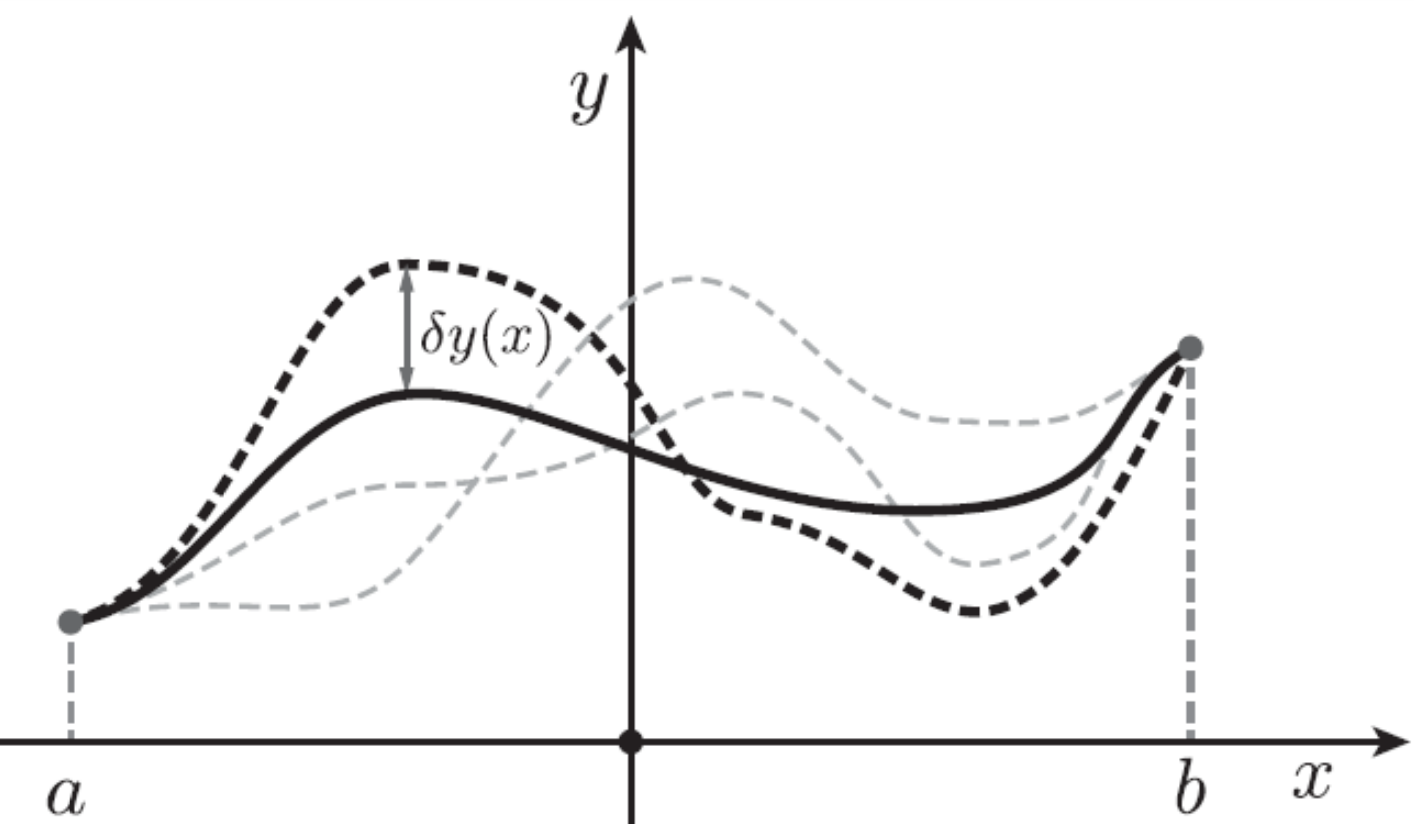
\includegraphics[width=1\textwidth]{Images/I_Function.PNG}\label{fig:f1}}
    \end{figure}   
    The variation of the function describes the summarization of Hamilton's principle. A vanishing variation of the line integral denotes a "stationary integral". The below formulation is abizmal, reference section \ref{} for better detail; Ultimately, we get equation \ref{eq: Euler}.
    \begin{equation}
        \delta I = \delta \int_{t_1}^{t^2} L(q_1, \dots, q_n, \dot{q}_1, \dots, \dot{q}_n, t) dt = 0
    \end{equation}
    \begin{equation}
        \delta I[y(x)] = I[y(x) + \delta y(x)] - I[y(x)] = 0
    \end{equation}
    Plug in I function definition
    \begin{equation}
        \delta I[y(x)] = \int_{x_a}^{x_b} \left( \frac{\partial F}{\partial y(x)} \delta y(x) + \frac{\partial F}{\partial y'(x)} \frac{d}{dx} (\delta y(x)) \right) dx = 0
    \end{equation}
    Integrate the equation and rearrange to get "Euler-Lagrange differential equation"
    \begin{equation} \label{eq: Euler}
        \boxed{\frac{\partial F}{\partial y(x)} - \frac{d}{dx} \left( \frac{\partial F}{\partial y'(x)} \right) = 0}
    \end{equation}
    For multiple ($N$) variable problems such as a point in space in 3D ($N=3$) we get 
    \begin{equation}
        \boxed{\frac{\partial F}{\partial y_i(x)} - \frac{d}{dx} \left( \frac{\partial F}{\partial (y_i)'(x)} \right) = 0} \text{ for } i = 1,\dot,N
    \end{equation}

    \begin{equation}
        S[q_k(t)] \equiv \int_{t_a}^{t_b} dt L(t,q_k,\dot{q}_k)
    \end{equation}

    Hamilton's principle: out of all possible paths by which the system point could travel from its position at time ($t_a$) to its position at time ($t_b$) it will actually travel along that path for which the value of the integral ins stationary
    \begin{equation}
        \delta S = \delta \int_{t_a}^{t_b} L(t,q_k,\dot{q}_k) dt = 0
    \end{equation}
    Hamiltonian equations
    \begin{gather*}
        \mathcal{H} = p \dot{q} - L = T + v
        \\ \frac{\partial L}{dt} = - \frac{d \mathcal{H}}{dt}
        \\ \dot{p} = \frac{\partial \mathcal{H}}{\partial q}
        \\ \dot{x} = \frac{\partial \mathcal{H}}{\partial p}
        \\ p = m \dot{x}
        \\ \dot{p} = 
    \end{gather*}

    Condition to verify that a function is ""
    \begin{equation}
        \nabla \cross \vec{F} = 0
    \end{equation}

    In general, nonholonomic constraints cannot be expressed by a variational principle. One of the exceptions is semi-holonimc constraints where the constrinats can be written as a set of functions of the form
    \begin{equation}
        f_\alpha(q_1, \dots, q_n, \dot{q}_1, \dots, \dot{q}_n, t) = \sum_{k=1}^n a_{ak} \dot{q}_k + a_0 = 0
    \end{equation}
    Where $a_{ak}$ and $a_0$ are functions of $q$ and $t$ and $f_\alpha$ is a set of nonintegrable differential expressions. We can't integrate the constraints.
    \begin{equation}
        \delta \int_{t_1}^{t_2} \left(\mathcal{L} + \sum_{\alpha = 1}^m \mu_a f_a \right) dt = 0
    \end{equation}
    $\mu$ is used to distinguish from holonomic Lagrange multipliers. Assume $\mu_a = \mu_a(t)$
    \begin{equation}
        \frac{d}{d t} \frac{\partial \mathcal{L}}{\partial \dot{q_k}} - \frac{\partial \mathcal{L}}{\partial q_k} = Q_k = - \sum_{a = 1}^m \mu_a \frac{\partial f_a}{\partial \dot{q}_k}
    \end{equation}
    The Lagrange undetermined multipliers method eliminates the extra virtual displacements
    \begin{equation}
        I = \int_1^2 \left(\mathcal{L} = \sum_{\alpha = 1}^m \lambda_\alpha f_a \right)
    \end{equation}
    Where $q_\alpha$ and $\lambda_\alpha$ vary independently to obtain n+m constraint equations, respectively. 
    %\newline \textcolor{red}{Actually, I don't think this matters. I am going to skip it, but if it comes up in an example I will return to this problem.}

    Lagrangian of a pendulum
    \[
        \mathcal{L} = T - V = \frac{1}{2} m \ell^2 \dot{\theta}^2 - m g \ell (1 - cos(\theta))
    \]
    Where $\ell$ is the length of the pendulum string

    Lagrangian of a double pendulum
    \[
        T = \frac{1}{2} m_1 \ell_1^2 \dot{\theta}_1^2 + \frac{1}{2} m_2 \left(\ell_1^2 \dot{\theta}_1^2 + \ell_2^2 \dot{\theta}_2^2 + 2 \ell_1 \ell_2 \dot{\theta}_1 \dot{\theta}_2 cos(\theta_1 - \theta_2) \right)
    \]
    \[
        V = m_1 g \ell_1 (1 - cos(\theta_1)) + m_2 g \left(\ell_1 (1 - cos(\theta)1) + \ell_2 (1 - cos(\theta_2)) \right)
    \]
    The motion of the double pendulum is chaotic for most initial conditions, making it an excellent example of a deterministic system that exhibits chaotic behavior. The equations of motion are highly coupled and nonlinear. 
    \begin{figure}[H]
        \centering
        \subfloat[Double-Pendulum]{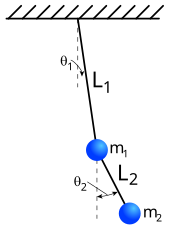
\includegraphics[width=0.5\textwidth]{Images/Double-Pendulum.png}\label{fig:f1}}
    \end{figure}

    Lagrangian of a pendulum with a moving pivot
    \[
        \mathcal{L} = \frac{1}{2} m \ell^2 \dot{\theta}^2 - m g \ell cos(\theta) - m a(t) \ell cos(\theta)
    \]
    Where $a(t)$ is the acceleration, vertically, of the pivot point.
    
    Lagrangian of a gravitating body
    \[
        \mathcal{L} = T - V = \frac{1}{2} m \left(\dot{r}^2 + r^2 \dot{\theta}^2 + r^2 sin^2(\theta) \dot{\phi}^2 \right) + \frac{G M m}{r}
    \]
    Where $G$ is the gravitational constant, $M$ is the mass of the source, $m$ is the mass of the probe, and $r$ is the radial distance between the source and the probe. Don't use this outright, because the effective potential is different. 

    Lagrangian of a charged particle in an electric and magnetic field (Lorentz force)
    \[
        \mathcal{L} = \frac{1}{2} m \dot{\vec{r}}^2 + q \dot{\vec{r}} \cdot \vec{A} - q \Phi
    \]
    Where $\vec{A}$ is the magnetic vector potential, $\Phi$ is the electric potential, $q$ is the charge. The equation of motion is
    \[
        m \ddot{\vec{r}} = q \left( \vec{E} + \dot{\vec{r}} \cross \vec{B} \right)
    \]

    
    Where $\vec{E}$ and $\vec{B}$ are the electric and magnetic fields. 

    Lagrangian of a harmonic oscillator
    \[
        \mathcal{L} = \frac{1}{2} m \dot{x}^2 - \frac{1}{2} k x^2
    \]
    The equation of motion is 
    \[
        m \ddot{x} + k x = 0
    \]
    

\section{Math}
    Calculus of Variations
    1-D Example, but shows the mathematical tool to variation
    We have a generic function ($f(y, \dot{y}, x)$), where $y$ is a function of $x$, and $\dot{y}$ is a derivative with respect to $x$, and we call the line integral of this equation $J$.
    \begin{gather*}
        \dot{y} \equiv \frac{dy}{dx}
        \\ J = \int_{x_1}^{x_2} f(y,\dot{y}, x) dx
    \end{gather*}
    We denote neighboring paths with $\alpha$ such as; $y(x,\alpha)$ for the general reference and $y(x,0)$ which represents the correct path. %\textcolor{red}{Skipping the function $\eta$}
    \begin{equation}
        J(\alpha) = \int_{x_1}^{x_2} f(y(x,\alpha), \dot{y}(x,\alpha), x) dx
    \end{equation}
    To obtain the stationary point
    \begin{equation}    
        \left(\frac{dJ(\alpha)}{d \alpha} \right) = 0
    \end{equation}
    Using Product Rule
    \begin{equation}
        \left(\frac{dJ(\alpha)}{d \alpha} \right) = \int_{x_1}^{x_2} \left(\frac{\partial f}{\partial y} \frac{\partial y}{\partial \alpha} + \frac{\partial f}{\partial \dot{y}} \frac{\partial \dot{y}}{\partial \alpha} \right) dx
    \end{equation}
    Consider only the second of these integrals and integrate by parts
    \begin{equation}
        \int_{x_1}^{x_2} \frac{\partial f}{\partial \dot{y}} \left( \frac{\partial \dot{y}}{\partial \alpha} \right) dx = \int_{x_1}^{x_2} \left( \frac{\partial f}{\partial \dot{y}} \frac{\partial^2 y}{\partial x \partial \alpha} \right) dx = \left( \frac{\partial f}{\partial \dot{y}} \frac{\partial y}{\partial \alpha} \right)_{x_1}^{x_2} - \int_{x_1}^{x_2} \frac{d}{dx} \left(\frac{\partial f}{\partial \dot{y}} \frac{\partial y}{\partial \alpha} \right)
    \end{equation}
    The partial derivative of $y$ with respect to $\alpha$ at $x_1$ and $x_2$ vanish. This is the condition that the two endpoints of the line are "set". 
    \begin{equation}
        \left(\frac{dJ(\alpha)}{d \alpha} \right) = \int_{x_1}^{x_2} \left(\frac{\partial f}{\partial y} - \frac{d}{dx} \frac{\partial f}{\partial \dot{y}} \right) \frac{\partial y}{\partial \alpha} dx
    \end{equation}
    Fundamental Lemma
    \begin{equation}
        \int M(x) \eta(x) dx = 0 \text{ For all arbitrary functions ($\eta(x)$ then } M(x) = 0
    \end{equation}
    The following equation represents a condition for finding curves continuous through the second derivative that render the integral stationary. 
    \begin{equation}
        \frac{\partial f}{\partial y} - \frac{d}{dx} \frac{\partial f}{\partial \dot{y}}
    \end{equation}
    Same thing for a plane
    \begin{equation}
        ds = \sqrt{dx^2 + dy^2}
    \end{equation}
    \begin{equation}
        I = \int_1^2 ds = \int_{x_1}^{x_2} \sqrt{1 + \left(\frac{dy}{dx} \right)^2} dx
    \end{equation}
    Where 
    \begin{equation}
        f = \sqrt{1 + \dot{y}^2}
    \end{equation}
    Same thing for a surface. Take the area of a strip of the surface 
    \begin{equation}
        2 \pi x ds = 2 \pi x \sqrt{1 + \dot{y}^2} dx
    \end{equation}

    Derivation that might be needed when determining equation of motion for plane
    We are given the function:
    \[
    f(y') = \sqrt{1 + (y')^2}
    \]
    To find the derivative of \( f(y') \) with respect to \( y' \), we can use the chain rule. 
    First, rewrite the function as a power of \( 1/2 \):
    \[
    f(y') = \left( 1 + (y')^2 \right)^{1/2}
    \]
    Now, apply the chain rule. The derivative of \( u^{1/2} \) with respect to \( u \) is \( \frac{1}{2} u^{-1/2} \), and we multiply this by the derivative of \( u = 1 + (y')^2 \).
    \[
    \frac{d}{dy'} \left( \left( 1 + (y')^2 \right)^{1/2} \right) = \frac{1}{2} \left( 1 + (y')^2 \right)^{-1/2} \cdot \frac{d}{dy'} \left( 1 + (y')^2 \right)
    \]
    Now, take the derivative of \( 1 + (y')^2 \):
    \[
    \frac{d}{dy'} \left( 1 + (y')^2 \right) = 2y'
    \]
    Substituting this into the expression, we get:
    \[
    \frac{d}{dy'} \left( \sqrt{1 + (y')^2} \right) = \frac{1}{2} \left( 1 + (y')^2 \right)^{-1/2} \cdot 2y'
    \]
    Simplify the expression:
    \[
    \frac{d}{dy'} \left( \sqrt{1 + (y')^2} \right) = \frac{y'}{\sqrt{1 + (y')^2}}
    \]
    Thus, the derivative of \( \sqrt{1 + (y')^2} \) with respect to \( y' \) is:
    \[
    \frac{y'}{\sqrt{1 + (y')^2}}
    \]
    
    
    
    

    
\section{Facts}
    Fermat proposed that out of all the infinite number of possible paths that a ray might take, it travels by the path of least time
    \newline Calculus of Variation or Functional Calculus is the method to minimize an integral
    \newline Hamilton's Principle describes the motion of those mechanical systems for which all forces (except the forces of constraint) are derivable from a generalized scalar potential that may be a function of the coordinates, velocities, and time. The motion of the system from time $t_1$ to time $t_2$ is such that the line integral (called the action or the action integral), where $L = T - V$, has a stationary value for the actual path of the motion.
    \newline Monogenic system: A physical system where the force acting on it can be modeled in a convenient mathematical form.
    \newline Stationary Integral: Integral along the given path has the same value to within first-order infinitesimals as that along all neighboring paths (those that differ from it by infinitesimal displacements).
    \newline Holonomic: A system in which one can deduce the state of a system by knowing only the change of positions, but not needing to know velocity, or how they move relative to each other. 
    \newline Theory of fields apparently describes non mechanical systems in the mathematical clothes of classical mechanics
    \newline Stationary integrals may not be minimum paths. In the case of a symmetric line, Eulers equation will not provide a solution
    \newline An advantage of the Lagrangian formulation is that it can be easily extended to describe systems that are not typically considered "dynamics", such as elastic fields, electromagnetic field, and the field properties of elementary particles. 
    \newline When a variation principle is used as the basis of the formulation, all such fields (Newtons equations, Maxwell's equations, Schrodinger equation, etc) will exhibit, at least to some degree, a structural analogy like we see between mechanical and electrical systems.  
    \newline The methods of quantization started essentially from the Lagrangian formulation of classical mechanics. By describing the electromagnetic field by a Lagrangian and corresponding Hamilton's variation principle, it is possible to carry over other methods of particle quantization to construct a quantum electrodynamics. 

\section{Variables}
    \begin{enumerate}
        \item $\vec{v} = $ Vector Velocity 
        \item $\vec{r} = $ Vector Radius
        \item $\vec{p} = $ Linear Momentum %\textcolor{red}{Vector?}
        \item $\vec{P} = $ Total Linear momentum of the system
        \item $\vec{F} = $ Total Force %\textcolor{red}{Vector?}
        \item $\vec{L} =$ Angular Momentum
        \item $\vec{N} = $ Moment of Force, Torque
        \item $T = $ Kinetic Energy
        \item $V = U = $ Potential Energy
        \item $L = $ Lagrangian
        \item $W_{12} = $ Work done by external force upon a particle going from point 1 to point 2
        \item $\vec{F}_{ji} = $ Internal force on the $i^{th}$ particle due to the $j^{th}$ particle
        \item $\vec{F}_i^{(e)}$ External force acting on the $i^{th}$ particle
        \item $\vec{F}^{(e)} = $ Total External force on the system of particles
        \item $\vec{R} = \frac{\sum_i m_i \vec{r}_i}{\sum_i m_i}$ Average of all particle radii vectors
        \item $\vec{r}' = $ Radius vector from the center of mass to the $i^{th}$ particle
        \item $\vec{r}'' = $ Radius vector from the origin to the center of mass. In the notes this is noted $\vec{R}$.
        \item $\vec{v}'' = $ Velocity of the center of mass relative to origin. In the notes this is notes $\vec{v}$
        \item $k = $ Number of equations in holonomic constraints
        \item $\vec{f} = $ Force of constraint in virtual work equation
        \item $Q_j = $ Generalized force (Not always a force unit)
        \item $t_p = $ Time taken for a photon to travle through a medium
        \item $c = $ Speed of light ()
        \item $S[q_k(t)] = $ Action of a mechanical system
    \end{enumerate}

\section{Examples}
    \subsection{Small object on hemisphere, Section 2.4, Pg 47}
    Consider a smooth solid hemisphere with radius ($r$). Place object with mass ($m$) on the top with an infinitesimal displacement off center.
    \begin{figure}[H]
        \centering
        \subfloat["]{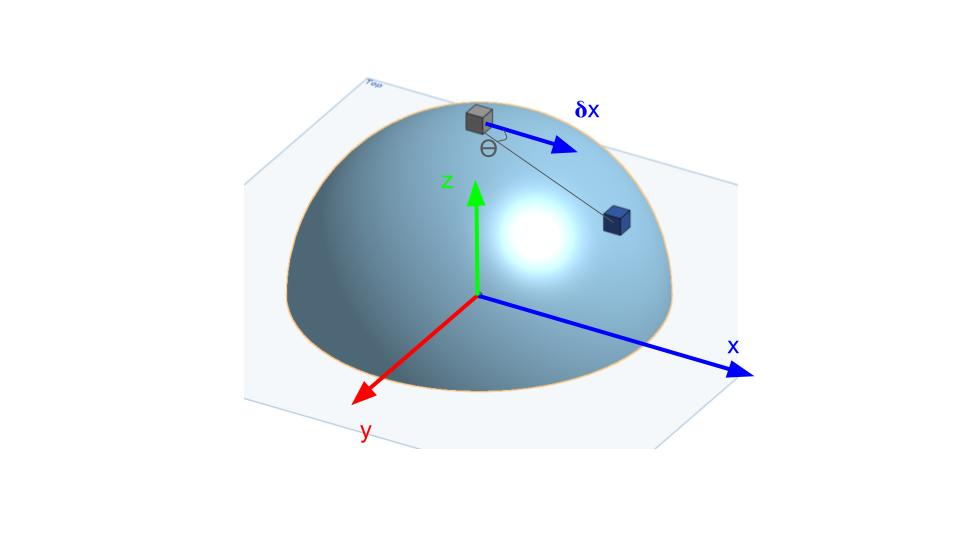
\includegraphics[width=1\textwidth]{Images/Example1.jpg}\label{fig:f1}}
    \end{figure}   
    The Lagrangian is 
    \begin{equation}
        \mathcal{L} = T - V = \frac{1}{2}m(\dot{x}^2 + \dot{y}^2 + \dot{z}^2) - m g z
    \end{equation}
    with Kinetic Energy ($T$), Potential Energy ($P$), and gravitational acceleration ($g$). All portions of the $y$ coordinate are removed because the infintesimal displacment is in the $x$ direction and gravity is in the $z$ direction. 
    \begin{gather*}
        r = \sqrt{x^2 + x^2} \text{ per pythagoreum}
        \\ \frac{x}{z} = cos(\theta) \text{ per trig relations "SOHCAHTOA"}
    \end{gather*}
    Lagrange Equations become
    %\newline \textcolor{red}{Do inbetween, maybe use Eulers derivative equation}
    %\newline \textcolor{red}{What is $\lambda$}
    \begin{gather*}
        m r \dot{\theta}^2 - m g cos(\theta) + \lambda = 0
        \\ m r^2 \ddot{\theta} + m g r sin(\theta) = 0
    \end{gather*}
    Solve the second equation then the first
    %\newline \textcolor{red}{Do inbetween}
    \begin{gather*}
        \dot{\theta}^2 = - \frac{2 g}{r} cos(\theta) + \frac{2 g}{r}
        \\ \lambda = m g (3 cos(\theta) - 2)
    \end{gather*}
    $\lambda$ is the magnitude of the force keeping the particle on the sphere. Once it reaches 0, the object will be in free fall. 
    \newline Since $\lambda = 0$ when $\theta = cos^{-1}(\frac{2}{3})$, the object leaves the sphere at that angle. 

    \subsection{Determine Particle motion given Lagrangian and nonholonomic constraint, Section 2.4, Pg 48}
    Given Lagrangian 
    \begin{equation}
        \mathcal{L} = \frac{1}{2} m (\dot{x}^2 + \dot{y}^2 + \dot{z}^2) - V(x,y,z)
    \end{equation}
    Given nonholonomic constraint
    \begin{equation} \label{eq: nonhom1}
        f(x,\dot{x}, y, \dot{y}, z) = \dot{x} y^2 + x \dot{y} + k z = 0
    \end{equation}
    Where $k$ is a constant. The equations of motion are:
    %\textcolor{red}{Do inbetween}
    \begin{equation} \label{eq: nonhom2}
        m \ddot{x} + \mu y^2 - \frac{\partial V}{\partial x} = 0
    \end{equation}
    \begin{equation} \label{eq: nonhom3}
        m \ddot{y} + \mu x - \frac{\partial V}{\partial y} = 0
    \end{equation}
    \begin{equation} \label{eq: nonhom4}
        m \ddot{z} - \frac{\partial V}{\partial z} = 0
    \end{equation}
    Where $\mu$ is a multiplier. Solve equations \ref{eq: nonhom1}, \ref{eq: nonhom2}, \ref{eq: nonhom3}, and \ref{eq: nonhom4} for variables $x(t)$, $y(t)$, $z(t)$, and $u(t)$.
    %\textcolor{red}{Do}

    \subsection{Hoop Rolling down a hill, Section 2.4, Pg 50}
    \begin{figure}[H]
        \centering
        \subfloat[A hoop rolling down an inclined plane]{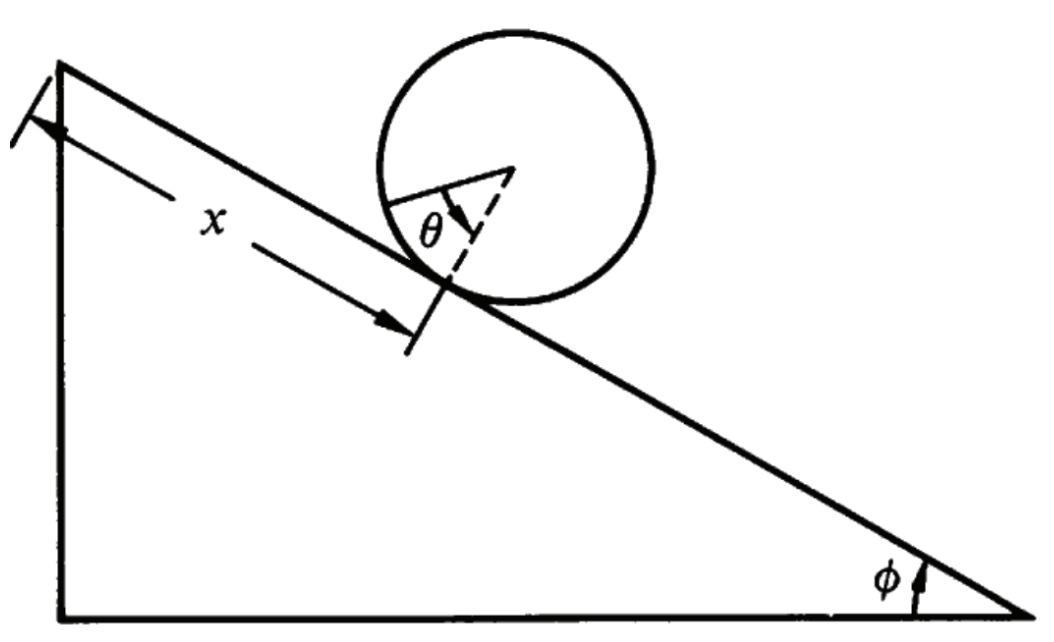
\includegraphics[width=1\textwidth]{Images/Ring_Down_Hill.JPG}\label{fig:f1}}
    \end{figure} 
    Assume generalized coordinates $x$ and $\theta$
    Assume that there is no slipping, which provides this a "rolling" constraint, which is holonomic. 
    \begin{equation}
        r d \theta = dx
    \end{equation}
    %\textcolor{red}{Do inbetween}
    \begin{equation} \label{eq: roll1}
        r \dot{\theta} = \dot{x}
    \end{equation}
    The Kinetic Energy ($T$) contains both translational and rotational
    \begin{equation}
        T = \frac{1}{2} M \dot{x}^2 + \frac{1}{2} M r^2 \dot{\theta}^2
    \end{equation}
    The Potential Energy ($V$) is dependent on gravity with respect to the incline
    \begin{equation}
        V = M g (l - x) sin(\phi)
    \end{equation}
    The Lagrangian is defined as 
    \begin{equation}
        \mathcal{L} = T - V = \frac{1}{2} M \dot{x}^2 + \frac{1}{2} M r^2 \dot{\theta}^2 - M g (l - x) sin(\phi)
    \end{equation}
    Since there is only one equation of constraint, only one Lagrange multiplier ($\lambda$) is needed. The constraint equation coefficients are:
    \begin{gather*}
        a_\theta = r
        \\ a_x = -1
    \end{gather*}
    The Lagrange equations are then 
    %\textcolor{red}{I should know this from ch 1 but I don't. Do inbetween}
    \begin{equation} \label{eq: roll2}
        M \ddot{x} - M g sin(\phi) + \lambda = 0
    \end{equation}
    \begin{equation} \label{eq: roll3}
        M r^2 \ddot{\theta} - \lambda r = 0
    \end{equation}
    Differentiate equation \ref{eq: roll1} with respect to time to isolate $\ddot{\theta}$
    \begin{equation}
        r \ddot{\theta} = \ddot{x}
    \end{equation}
    \begin{equation}
        \ddot{\theta} = \frac{\ddot{x}}{r}
    \end{equation}
    Plug into equation \ref{eq: roll3}
    \begin{equation}
        M r^2 \left(\frac{\ddot{x}}{r} \right) - \lambda r = 0
    \end{equation}
    Isolate $M \ddot{x}$ to plug into equation \ref{eq: roll2}
    \begin{gather*}
        M r^2 \left(\frac{\ddot{x}}{r} \right) = \lambda r\ddot{x}
        \\ M r \ddot{x} = \lambda r
        \\ M \ddot{x} = \lambda
        \\ M \ddot{x} - M g sin(\phi) + M \ddot{x} = 0
    \end{gather*}
    Isolate $\ddot{x}$
    \begin{gather*}
        M \ddot{x} - M g sin(\phi) + M \ddot{x} = 0
        \\ 2 M \ddot{x} = M g sin(\phi)
        \\ \ddot{x} = \frac{g sin(\phi)}{2}
    \end{gather*}
    Plug into \ref{eq: roll2} to get $\lambda$ (The friction force of constraint)
    \begin{gather*}
        M \left(\frac{g sin(\phi)}{2} \right) - M g sin(\phi) + \lambda = 0
        \\ \lambda = \frac{M g sin(\phi)}{2}
    \end{gather*}
    Plug into equation \ref{eq: roll3} to get $\ddot{\theta}$ 
    \begin{gather*}
        M r^2 \ddot{\theta} - \left(\frac{M g sin(\phi)}{2} \right) r = 0
        \\ \ddot{\theta} = \frac{M g r sin(\phi)}{2 M r^2} =  \frac{g sin(\phi)}{2 r}
    \end{gather*}
    Conclusion: The hoop rolls down the incline with only one-half the acceleration it would have slipping down a friction-less plane.

    \subsection{Battery, Section 2.5, Pg 52}
    A battery with Voltage ($V$) in series with an inductor ($L$) and resistor ($R$) with the electric charge ($q$) as the dynamic variable. 
    The Kinetic Energy of the Inductor ($T_i$)
    \begin{equation}
        T_i = \frac{1}{2} L \dot{q}^2
    \end{equation}
    The dissapative function from the Resistor ($\mathcal{F}$)
    \begin{equation}
        \mathcal{F} = \frac{1}{2} R \dot{q}^2
    \end{equation}
    %\textcolor{red}{Do inbetween. Get Lagrangian and determine equation of motion}
    The equation of motion
    \begin{equation}
        V = L \ddot{q} + R \dot{q} = L \dot{I} + R I
    \end{equation}
    Where the electric Current ($I = \dot{q}$). 
    \newline This is the solution to the equation of motion.
    %\newline \textcolor{red}{I guess this is a mathematical solution to the differential equation of motion}
    A solution for a battery connected to the circuit at time ($t=0$)
    \begin{equation}
        I(t) = I_0 (1 - e^{-\frac{R t}{L}}
    \end{equation}
    Where $I_0 = \frac{V}{R}$ %\textcolor{red}{Again, just circuits knowledge}

    \subsection{Sphere in fluid, Section 2.5, Pg 52}
    A sphere of radius ($r$) is falling in a viscous fluid of constant density ($\rho$) and viscosity ($\eta$) under the force of gravity. The effective mass ($m'$) is the difference between the actual mass of the sphere and the mass of the displaced fluid. 
    \newline The Kinetic Energy of the sphere falling due to gravity ($T_g$)
    \begin{equation}
        T_g = \frac{1}{2} m' \dot{y}^2
    \end{equation}
    The dissipative function from frictional drag ($\mathcal{F}$) where the force of the frictional drag is $F_f = 6 \pi \eta r \dot{y}$
    \begin{equation}
        \mathcal{F} = \frac{1}{2} F_f \dot{y} = 3 \pi \eta r \dot{y}^2
    \end{equation}
    The potential energy of the sphere ($P_s$)
    \begin{equation}
        P_s = m' g y
    \end{equation}
    %\textcolor{red}{Do inbetween. Get Lagrangian and determine equation of motion}
    The equation of motion is 
    \begin{equation}
        m' g = m' \ddot{y} + 6 \pi \eta r \dot{y}
    \end{equation}
    %\newline \textcolor{red}{I guess this is a mathematical solution to the differential equation of motion}
    A solution for the sphere traveling from rest ($t=0$)
    \begin{equation}
        \dot{y} = \dot{y}_0 (1 - e^{-\frac{t}{\tau}}
    \end{equation}
    Where $\tau = \frac{m'}{6 \pi \eta r}$ is the time it takes the sphere to reach terminal speed ($\dot{y}_0 = \frac{m' g}{6 \pi \eta r}$)

    \subsection{Inductor in series with Capacitor, Section 2.5, Pg 53}
    And inductor ($L$) is in series with a Capacitor ($C$)
    The Kinetic Energy of the Inductor ($T_i$)
    \begin{equation}
        T_i = \frac{1}{2} L \dot{q}^2
    \end{equation}
    The potential energy of the Capacitor ($P_c$)
    \begin{equation}
        P_c = \frac{q^2}{C}
    \end{equation}
    where the electrical charge ($q$)
    %\textcolor{red}{Do inbetween. Get Lagrangian and determine equation of motion}
    The equation of motion is
    \begin{equation}
        L \ddot{q} + \frac{q}{C} = 0
    \end{equation}
    %\newline \textcolor{red}{I guess this is a mathematical solution to the differential equation of motion}
    A solution for the charged capacitor from start ($t=0$) assuming no charge is flowing at the start so the charge that is already stored in the capacitor ($q_0$)
    \begin{equation}
        q = q_0 cos(\omega_0 t)
    \end{equation}
    Where the resonant frequency of the system is
    \begin{equation}
        \omega_0 = \frac{1}{\sqrt{L C}}
    \end{equation}

    \subsection{Simple Harmonic Oscillator, Section 2.5, Pg 53}
    A simple harmonic oscillator is described by the Lagrangian
    \begin{equation}
        \mathcal{L} = \frac{1}{2} m \dot{x}^2 - \frac{1}{2} k x^2
    \end{equation}
    %\textcolor{red}{Do inbetween}
    The equation of motion 
    \begin{equation}
        m \ddot{x} + k x = 0
    \end{equation}
    %\newline \textcolor{red}{I guess this is a mathematical solution to the differential equation of motion}
    A solution for the oscillating mass from the start ($t=0$)
    \begin{equation}
        x = x_0 cos(\omega_0 t)
    \end{equation}
    \begin{equation}
        \omega_0 = \sqrt{\frac{k}{m}}
    \end{equation}

    \subsection{Coupled electronics, Section 2.5, Pg 54}
    \begin{figure}[H]
        \centering
        \subfloat[Example Coupled Curcuit]{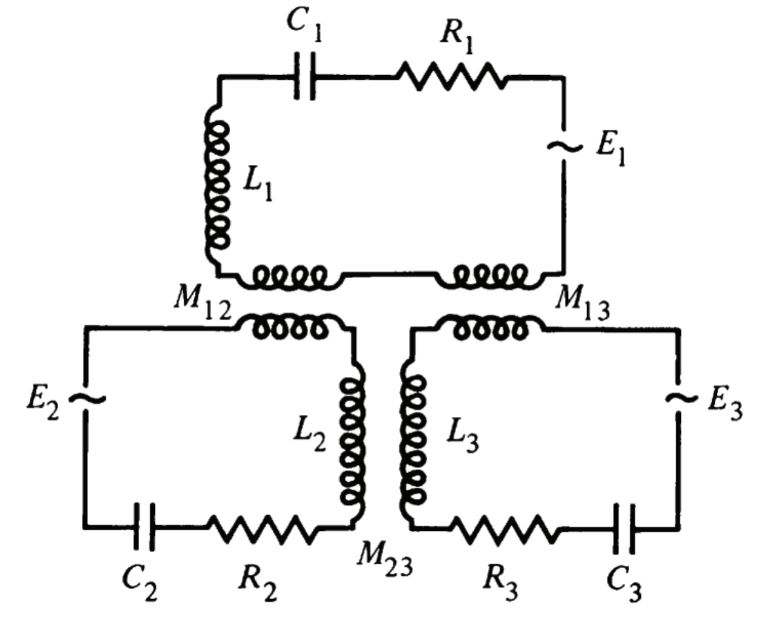
\includegraphics[width=1\textwidth]{Images/Coupled_Curcuit.JPG}\label{fig:f1}}
    \end{figure}
        The Lagrangian is 
    \begin{equation}
        \mathcal{L} = \frac{1}{2} \sum_j L_j \dot{q}_j^2 + \frac{1}{2} \sum_{jk, j \neq k} M_{jk} \dot{q}_j \dot{q}_k - \sum_j \frac{q_j^2}{2 C_j} + \sum_j e_j(t) q_j
    \end{equation}
    The dissipative function from the Resistors ($\mathcal{F}$)
    \begin{equation}
        \mathcal{F} = \frac{1}{2} \sum_j R_j \dot{q}_j^2
    \end{equation}
    The lagrange equations %\textcolor{red}{does this mean "equations of motion"}
    \begin{equation}
        L_j \frac{d^2 q_j}{dt^2} + \sum_{k,j \neq k} M_{jk} \frac{d^2 q_j}{dt} + R_j \frac{d q_j}{dt} + \frac{q_j}{C_j} = E_j(t)
    \end{equation}
    Where $E_j(t)$ is the external emf of the system and $e_j(t)$ is the external emf of each individual charge
    
    
    






































    
\newpage
%\printbibliography
\end{document}
